\documentclass[a4paper,12pt]{article}
\usepackage[french]{babel}
\usepackage[T1]{fontenc}
\usepackage[utf8]{inputenc}
\usepackage{graphicx}
\usepackage{pdfpages}
\usepackage{fancyhdr}
\pagestyle{fancy}
\fancyhead[L]{PAO Nao joue à pong}
\fancyhead[R]{ASI 3.2 - INSA Rouen}
\fancyfoot[L]{GICQUEL - MARTIN - THEOLOGIEN}
\fancyfoot[R]{\thepage}
\fancyfoot[C]{}

\newcommand{\pao}{\textit{Projet d'Approfondissement et d'Ouverture}}
\newcommand{\projet}{\textit{Nao joue à Pong}}


\begin{document}
\begin{titlepage}
\thispagestyle{empty}
\begin{figure}
	\includegraphics[width=5cm]{Images/Insa.png}\hfill
	\includegraphics[width=5cm]{Images/ASI.png}\
\end{figure}

\newcommand{\HRule}{\rule{\linewidth}{0.5mm}} 
\center 
\vspace*{\stretch{1}}\textsc{\huge Institut National des Sciences Appliqu\'{e}es de Rouen}\\[1.5cm] 
\textsc{\Large Projet d'Approfondissment et d'Ouverture}\\[2cm] 

\HRule \\[0.4cm]
{ \huge \bfseries Nao joue à Pong}\\[0.2cm] 
\HRule \\[2.5cm]
  


\large \emph{\textbf{Auteurs :}}\\
	Enora GICQUEL\\
	Florian MARTIN\\
	Thibault THEOLOGIEN \\

~\\ ~\\[1cm]

\vfill{\today}\\[3cm]

\end{titlepage}

	\pagebreak
	\tableofcontents
	\pagebreak

	\section{Introduction}
\label{sec:Introduction}

\par Lors de ce semestre d'ASI 3.2, nous avions la possibilité de suivre un \pao.
Nous avons repris le sujet \projet\ qui a débuté au semestre précédent sous la direction de Monsieur Nicolas Delestre.

\par Nous avons choisi ce sujet afin d'appliquer nos compétences en développement informatique dans un contexte nouveau, à savoir la robotique.
Nous étions également intéressés par la découverte d'outils de programmation pour une utilisation assez ludique.

\par Ce rapport présente l'évolution du projet au cours de ce semestre.
Nous commencerons par analyser le projet tel que nous l'avons repris, pour ensuite présenter nos objectifs pour cette succession.
Nous étudierons la conception relative au sujet puis son développement. Nous évoquerons également les différentes présentations que nous avons pu faire dans le cadre du projet.
Nous détaillerons aussi les problèmes rencontrés tout au long de la réalisation du projet.
Et nous finirons sur les évolutions possibles en cas de reprise du sujet.


\pagebreak

	\section{Etude de l'existant}
\label{sec:Etude de l'existant}
\par Nous avons eu comme base le code produit par une équipe auparavant qui avait pour 
but de produire une version permettant de confirmer la faisabilité du projet. Leur travail 
s'articulait autour de deux grands points qui sont l'IA et principalement la reconnaissance.

    \subsection{Reconnaissance}
    \par Au niveau de la reconnaissance, ces derniers ont produits différents modules de 
    reconnaissance. Ainsi ces différentes méthodes allaient de la comparaison d'histogramme, 
    qui se trouvait être peu fonctionnelle et offrait trop souvent de faux positifs au niveau 
    de la reconnaissance. Une autre méthode qui a été celle retenue consistait en l'utilisation 
    de la bibliothèque OpenCV, spécialisée dans le traitement d'images en temps réel, afin de 
    trouver les contours et formes des images afin de détecter les différents éléments du jeu de Pong.
    
    \par Cette méthode retenue offrait la plupart du temps une bonne reconnaissance du terrain,
    ainsi que des différents éléments du jeu de Pong, mais avait pour défaut majeur un très long 
    temps de traitement. Ainsi, la contrainte de réaction en temps réel du robot pour pouvoir jouer 
    correctement ne pouvait pas être respectée, le traitement durant environ 2 à 3 secondes pour réagir.
    
    \subsection{IA}
    \par L'IA qui a tout d'abord été implémentée était très basique. En effet cette dernière se contentait 
    de suivre la balle sur l'axe vertical avec la raquette. De plus la prise en compte du temps pour atteindre 
    la même hauteur que la balle n'était pas présente, le Nao se contentait donc de se déplacer par accoups afin 
    d'atteindre la position voulue après plusieurs reconnaissances effectuées.
    
    \par Malheureusement, du fait de la lenteur de la reconnaissance, cette solution n'était pas viable 
    pour faire jouer correctement le robot au Pong. Il arrivait donc de temps en temps que le Nao arrivait à 
    atteindre la balle à temps.
    
    \subsection{Structure globale du code}
    \par Le but étant de produire une version permettant de confirmer la faisabilité du projet, 
    le code produit ne suivait pas une structure modulaire, était difficilement maintenable et 
    compréhensible dans l'état dans lequel il se trouvait. Ainsi, les différents appels au robot 
    étaient effectués autant au niveau de l'IA que de la reconnaissance, ce qui rendait le code 
    très difficilement débuggable du fait de la dispersion des traitements dans les différentes 
    parties du code.
    
    \par Nous trouvions donc trois fichiers principaux qui étaient les fichiers Controle, IA et Reconnaissance.

\pagebreak

	\section{Presentation du projet}
\label{sec:Presentation du projet}

\pagebreak

	\section{Conception}
\label{sec:Conception}
  \par Se référer à l'annexe \ref{sec:Diagramme de classes} page \pageref{sec:Diagramme de classes} pour consulter le diagramme de classes. \\
  \par Se référer à l'annexe \ref{sec:Diagramme de séquence} page \pageref{sec:Diagramme de séquence} pour consulter le diagramme de séquence.
\pagebreak

	\section{Développement}
\label{sec:Développement}
  \subsection{Main}
\label{sub:Main}

  \par Le script main permet l'execution de l'ensemble du projet.
  Il prend en paramètre une adresse IP sous la forme d'une chaine de caractères, et eventuellement un port.
  Dans le cas ou le port ne serait pas renseigné, un port par défaut est attribué.
  Cette adresse IP correspond à celle du NAO sur le réseau local.\\
  La première étape consiste donc à initialiser le robot, et lui appliquer sa position de jeu.\\
  Ensuite, il faut déterminer la vitesse de déplacement en pixels par secondes de la barre controlée par le NAO.
  Pour cela, la capture de deux images, interrompues par une action du bras du NAO d'une durée suffisante (une seconde dans notre cas), puis leur traitement est necessaire. \\
  A l'issue de ce traitement, le NAO peut réellement commencer à jouer.
  Pour cela, les éléments du jeu sont récupérés, par la fonction traitement(nao, reconnaissance) du script courant, et envoyés à une fonction de l'IA.
  Cette dernière retournera une action (du bras du NAO), qui sera renvoyée au NAO.

  \par Deux fonctions sont utilisées dans ce script.
  La première, getImage(nao, reconnaissance) permet, à partir d'une classe nao et reconnaissance initialisée d'effectuer une capture d'image par le NAO ainsi que de détecter le terrain.
  Tant que le NAO ne détécte pas le terrain sur la photo, une nouvelle prise est effectuée.
  L'image découpée du terrain, ainsi qu'un objet terrain sont retournés par cette fonction.\\
  La seconde, traitement(nao, reconnaissance) permet, à partir des mêmes objets que la fonction précédente, de recuperer tous les éléments essentiels au jeu (barres, balle et terrain).
  En effet cette fonction appelle getImage(nao, reconnaissance), et à partir des objets retournés, appelle la fonction de la classe reconnaissance permettant la detection des éléments du terrain.
  Tant que tous les éléments du terrain ne sont pas détéctés, toute la procédure énuméré reprend à zéro, sinon les éléments du jeu sont retournés.

  \subsection{Module element}
\label{sub:Module element}
  \par Ce module est composé de classes de descriptions des éléments du jeu.
  Celles ci n'intègrent donc aucun comportement, et leur présence ne se justifie que d'un point de vu conceptuel.\\
  Les classes le composant sont donc \textit{Balle}, \textit{Barre}, \textit{Terrain} et \textit{Coordonnee}.

  \subsection{Module reconnaissance}
\label{sub:Module reconnaissance}
\par Afin de pouvoir prendre des décisions le Nao devait pouvoir tirer les informations nécessaires à partir de l'image qu'il prend.
\par La première étape est de détecter le terrain afin de concentrer la détection seulement sur la zone utile. La seconde étape consiste à déterminer les positions des éléments du jeu, donc la balle et les deux barres.
  \subsubsection{Détection terrain}
\label{subs:Détection terrain}
\par L'utilisation qui avait été faite d'OpenCV pour la détection du contour du
terrain par la précédente équipe n'était que
peu précise, peu rapide et renvoyait les contours extérieurs du terrain. Nous avons donc
travaillé sur la récupération des contours intérieurs du terrain de manière
suffisament sûre et rapide en accord avec les contraintes de temps d'exécution du projet.
\par Nous avons donc réussi à faire en sorte d'obtenir ce que nous voulions en
un temps suffisament faible pour permettre au robot d'agir dans un temps
acceptable. Notre méthode consiste en la détection à l'aide d'OpenCV d'un
rectangle ayant une taille minimale fixée afin de ne pas détecter les éléments
du terrain, on découpe grossièrement l'image de sorte à inclure le rectangle
détecté, puis on répète l'opération jusqu'à ne plus détecter de rectangle. Enfin
on recadre le dernier rectangle obtenu de sorte à ne plus avoir de
perspective sur l'image et faciliter le traitement.
\par On peut voir un exemple du résultat sur les figures 1 et 2.
\begin{figure}[h]
    \begin{minipage}[c]{.46\linewidth}
        \centering
        \includegraphics[width=7cm]{Images/reco1.jpg}
        \caption{Image avant recadrage du terrain}
    \end{minipage}
    \hfill%
    \begin{minipage}[c]{.46\linewidth}
        \centering
        \includegraphics[width=7cm]{Images/reco2.jpg}
        \caption{Image après recadrage du terrain}
    \end{minipage}
\end{figure}


  \subsubsection{Détection éléments}
\label{subs:Détection éléments}
\par La détection des éléments a été une étape délicate. Plusieurs techniques ont donc été testées afin de définir la meilleure en terme de rapidité et de précision.

\subsubsubsection{Technique de détection par forme}
\par Une première idée, un peu simpliste, était de détecter les éléments par leur forme. 
\par Pour cela on détectait les contours présents dans l'image et on définissait les formes que l'on recherchait : des rectangles plus haut que large pour les barres, et un petit carré pour la balle.
\par Cette technique était très rapide mais très aléatoire quant à la détection. En effet selon la précision des images  les éléments recherchés ne pouvaient être considérés comme des rectangles.

\subsubsubsection{Technique de détection par soustraction de contours}
\par Une autre idée était de soustraire les contours de deux images consécutives afin de récupérer les éléments ayant bougé entre celles-ci.
\par Quelques traitements supplémentaires étaient nécessaires pour différencier la balle des barres, mais globalement la détection était bonne et le traitement rapide.
\par Cette solution nous gênait cependant par certains aspects. Notamment la nécessité d'avoir pris deux images pour pouvoir effectuer le traitement, sachant qu'il faut deux détections pour déterminer le mouvement de la balle, la première réaction aurait été assez lente. Un autre point gênant se posait lorsque le score changeait puisque les contours dans cette zone changeait.

\subsubsubsection{Technique de détection par zone et par aire}
\par Une autre technique consistait à détecter les éléments selon leur zone et leur aire.
\par Cette solution part du principe que l'on connait à peu près la position x des barres puisque l'on cherche les éléments dont les contours donnent l'aire la plus grande dans les 2 extrémités du terrain. La détection de la balle se fait par recherche sur tout le terrain de l'élément ayant l'aire la plus petite et dont le point central est de couleur blanche (test de couleur dû à l'affichage du score).
\par La ligne centrale du terrain posant problème, on a choisi une petite proportion de la partie centrale du terrain.
\par Cette solution était rapide et la détection des éléments étaient bonnes sauf dans certains cas où ils étaient collés au bord du terrain. Dans le cas de la balle ce n'est pas très handicapant puisque cette configuration apparait beaucoup moins souvent que pour les barres qui posent plus problème.

\subsubsubsection{Technique de détection des éléments par moyennes et seuils}
\par Une fois le terrain obtenu et recadré nous avons travaillé sur une
technique permettant de détecter de manière presque sûre les différents éléments
présents sur le terrain. Ainsi cette technique consiste à contraster tout
d'abord le terrain en définissant les pixels de l'image à la couleur noire en
dessous de la valeur 128, et blanche au dessus. Ensuite nous parcourons les
côtés de l'image en essayant de trouver une région de pixels correspondant aux
éléments (Moyenne de blanc sur les lignes et colonnes de l'image afin de récupérer les
coordonnées et la taille des éléments). Ainsi nous avons pu observer avec notre
technique que nous obtenons correctement les coordonnées des barres dans la
majorité des cas (Nous avons pu observer lors de nos derniers essais quelques
ratés où l'une des barres n'était pas détectée), mais nous n'obtenions pas de
résultats satisfaisants concernant la détection de la balle.

\subsubsubsection{Choix final}
\par Finalement la solution retenu est un mélange de la détection par aire pour
la balle, et de la détection par moyennes et seuils pour les barres.
\par Ainsi on arrive à une détection assez précise et rapide.


  \subsection{Module IA}
\label{sub:Module IA}
\par Nous avons décidé pour ce PAO d'améliorer l'IA du Nao qui se contentait
auparavant de s'aligner selon l'axe vertical avec la balle.

\par L'IA que nous avons dévellopée suit des règles simples qui sont les
suivantes :

\begin{itemize}
	\item Si la balle se dirige vers la barre adverse, l'action renvoyée doit
		permettre au Nao de se positionner au milieu du terrain selon l'axe
		vertical.
	\item Sinon à l'aide de deux positions de la balle, l'angle de déplacement
		de celle-ci est calculé, puis la position où cette dernière est censée
		arriver au final. Ainsi l'IA peut être capable de se positionner
		correctement.
\end{itemize}

\par Nous avons admis qu'un rebond sur un mur avait pour effet sur l'angle de
l'inverser verticalement (Exemple: Un angle de 45° devient 135°).

\par Du fait de notre conception, où il a été décidé que le robot devait
prendre un temps de montée ou de descente pour agir, l'IA renvoie l'action correspondante
à l'indication de montée ou descente pendant un certain temps.
Pour cela il lui est nécessaire de calculer le temps de l'action afin
d'atteindre la position voulue.

\par Il s'est révélé par la suite que la vitesse passée à l'IA que nous obtenons ne
semble pas cohérente, ce qui fausse en partie les résultats pour l'action. De plus 
le comportement donné dans le programme principal (Calcul avec la précédente balle
qui a fait l'objet d'un traitement avec la plus récente détectée) ne permet pas 
d'obtenir régulièrement des résultats cohérents à cause des rebonds et des remises 
en jeu qui faussent le déplacement de la balle.
  \subsection{Module controle}
\label{sub:Module controle}
  \par Ce module est composé de deux classes, la première étant IP et la seconde NAO.

  \par La classe IP est en quelque sorte une classe de description puisqu'elle n'intègre aucun comportement spécifique, et a pour unique vocation de permettre la connexion au NAO d'une manière moins naïve.
  Sa présence se justifie essentiellement d'un point de vu conceptuel.

  \par C'est à partir de la classe NAO que toutes les instructions données au NAO (physique) sont exécutées.
  Cette classe est initialisée à partir d'une classe IP passée en paramètre, correspondant à celle du NAO sur le réseau local.
  De par le fait que peu d'actions sur le NAO ne sont requises pour ce projet, on ne retrouve qu'un nombre de fonctions assez limité dans cette classe, chacune correspondant à une action désirée.
  Les actions du NAO possibles à partir de notre module sont:
  \begin{itemize}
    \item appliquer la position initiale (on appelle la fonction correspondante au début du programme).
    Le robot est placé dans une position assise, avec le joystick dans la main, et avec la tête un peu inclinée sur le côté afin d'avoir un champ de vision assez large (sinon le bras tenant le joystick est visible).
    \item actionner le bras tenant le joystick (toujours le droit dans notre cas) dans une direction choisie, et pour une durée de temps déterminée.
    C'est par cet intermédiaire que l'on fait "jouer" le NAO.
    \item capturer une image, afin de permettre son traitement par le module de reconnaissance puis son interprétation à partir du module IA.
    Cette action requiert d'avoir préalablement initialisé la caméra du NAO, et de la couper à la fin du programme.
    \item parler, qui permet de faire "lire" au NAO une chaine de caractère.
    Cette fonctionnalité est assez secondaire dans ce projet, cependant elle permet de rentre le résultat final un peu plus attractif/vivant.
  \end{itemize}
\pagebreak

  \subsection{Module action}
\label{sub:Module action}
\par Ce module est composé de classes décrivant les actions à réaliser par le Nao. Aucun comportement n'y est intégré, son but étant essentiellement conceptuel.
\par Les classes présentes sont :
\begin{itemize}
\item \textit{direction} qui énumère les différentes directions vers lesquelles les mouvements peuvent être effectués, donc HAUT et BAS;
\item \textit{action} qui décrit l'action à effectuer en précisant sa direction et sa durée.
\end{itemize}
  \subsection{Module de statistiques des performances des reconnaissances}
\label{sub:Module de statistiques des performances des reconnaissances}

  \subsection{Module nao\_camera\_helper}
\label{sub:Module nao_camera_helper}

  \subsection{Module nao\_reco\_tester}
\label{sub:Module nao_reco_tester}
\par Au cours de notre développement, deux méthodes de reconnaissance ont fait leur apparition. Afin
de tester ces deux méthodes. Un ensemble d'images de tests où les positions étaient connues nous a donc
été fourni.

\par Afin d'effectuer nos tests, nous avons donc développé un outil (Fichier statistique\_reconnaissance.py)
nous permettant de récupérer les différentes erreurs produites par notre reconnaissance dans un fichier au format
CSV. Les données sauvegardées dans le fichier CSV sont les suivantes :

\begin{itemize}
    \item Chemin vers l'image;
    \item Erreur pour la balle sur l'axe horizontal;
    \item Erreur pour la balle sur l'axe vertical;
    \item Erreur pour la barre gauche;
    \item Erreur pour la barre droite;
    \item Erreur globale moyenne;
    \item Temps mis pour la reconnaissance du terrain;
    \item Temps mis pour la reconnaissance des éléments
\end{itemize}

\par Il c'est avéré que les données qui nous avaient été fournies ne correspondaient pas aux positions sur les images.
Il nous était donc impossible d'effectuer des tests avec celles-ci.

\par Nous avons donc décidé de développer une deuxième version de l'outil (Fichier nao\_capture\_pong.py). L'objectif
de cette deuxième version est de générer des états d'un jeu de Pong où les coordonnées sont connues et de faire en
sorte que le Nao prenne une image du terrain et effectue sa reconnaissance. Ainsi nous obtenons les données nous
permettant de calculer l'erreur produite par nos méthodes de reconnaissances.

\par Malheureusement, il ne nous a pas été possible de terminer cette version de l'outil du fait du temps qui nous était
imparti pour effectuer le projet. Nous avons donc préféré concentrer nos efforts sur des points plus importants du
projet. Ainsi, l'outil dans sa deuxième version est actuellement capable de générer un état du jeu
(À l'aide de la librairie PyQt4).
La partie manquante étant la capture d'image par le robot ainsi que l'enregistrement des données. Le programme devra donc prendre à terme
en tant que paramètre l'IP du Nao.

\par L'éxecution de ces outils se fait à partir du dossier 'nao' à l'aide des commandes suivantes :
\begin{center}
	{python2 chemin\_vers\_statistique\_reconnaissance.py [IP du Nao]}
\end{center}
\begin{center}
	{python2 chemin\_vers\_nao\_capture\_pong.py [IP du Nao]}
\end{center}

\par Concernant le premier programme, il est a noté que les images doivent se situer dans le dossier \'nao\' afin de
fonctionner.

\pagebreak

	\section{Présentation du projet à des élèves extérieurs}
\label{sec:Présentation du projet à des élèves extérieurs}
  \par Au cours des deux derniers mois du \pao\ nous avons eu l'occasion de présenter à deux reprises notre projet devant des élèves extérieurs.\\

  \subsection{Présentation du 22 avril}
  \label{sub:Présentation du 22 avril}
    \par La première présentation a eu lieu face à des élèves de seconde visitant l'établissement.
    Pour l'occasion, un diaporama expliquant rapidement et de la manière la plus simple le but de notre travail a été conçu.\\
    Nous avons fait le choix d'utiliser le framework JavaScript Reveal.js, pour ce diaporama.
    Ce framework permet de faire des presentations interactives de manière relativement aisée en HTML / CSS, puis de les visualiser depuis son navigateur.
    Cependant comme nous ne l’avions pas utilisé depuis un moment, cela a nécessité un certain temps de réadaptation.
    L'avantage de cette solution est qu'elle nous permettait d'utiliser un dépôt git, facilitant la mise en commun et les mises à jour de notre travail.\\
    \par Trouver comment aborder le sujet du projet pour la présentation devant les lycéens et essayer d’adapter son discours en conséquence n’a pas été si aisé.
    De plus, une démonstration du NAO jouant à Pong était requise.
    Cependant, à la date de la présentation, le projet était encore loin de son résultat final, et le code que nous avions ne nous permettait pas de faire une démonstration convenable de notre travail.
    Nous avons donc été contraints de réutiliser le travail effectué par les élèves travaillant avant nous sur ce PAO.\\

  \subsection{Présentation du 10 mai}
  \label{sub:Présentation du 10 mai}
    \par La seconde présentation s'est déroulée devant des élèves en CM1/CM2. \\
    Dans le cadre d'un projet personnel (Chimie Kids) des étudiants en CFI3 nous ont contactés afin que nous leur présentions le département ASI ainsi que notre PAO.
    Cette présentation étant de courte durée et face à d'aussi jeunes élèves, aucun diaporama n'était requis.
    Nous avons quand même dû donner quelques explications et il se trouve qu'adapter notre discours pour les écoliers s'est révéler encore plus difficile que lors de la présentation face aux lycéens.
    Nous avons également dû effectuer une démonstration du NAO jouant à Pong.
    Cette fois, notre avancement dans le projet nous a permis d'utiliser notre code.
\pagebreak

	\section{Problèmes rencontrés}
\label{sec:Problèmes rencontrés}

  \par Au cours de ce projet nous nous sommes retrouvé face à un certain nombre de difficultés, dans des domaines assez variés compte tenu de l'évolution du projet.
  En effet, les problèmes que nous avons pu rencontrer au cours des premières semaines concernaient plus des problèmes matériels,
  tandis que ceux rencontrés durant les dernières semaines étaient plus de l'ordre de contraintes de développement.\\
  Les sous-parties suivantes traiterons donc, par ordre chronologique, de ces problèmes auxquels nous avons dû faire face, ou que nous avons simplement indentifiés.\\

  \subsection{Semaines du 18 janvier au 1 fevrier}
    \label{sub:Semaines du 18 janvier au 1 fevrier}
    \begin{itemize}
      \item Les dépendances du projet ne nous ayant pas été fournies, nous avons dû les récupérer directement depuis internet.
      Or l'API NaoQI, indispensable pour interagir avec le robot, necessite l'obtention d'un statut de développeur au sein de la plateforme aldebaran, statut qui nous a été assez difficile à obtenir.
      \item Nous avons mis un certain temps à nous appercevoir que l'API NaoQI repose sur une ancienne version du langage Python (2.7).
      % NOTE: Flo t'as certainement un truc à ajouter ici pour les contraintes que ça a pu apporter
      \item Le code fourni n'était pas fonctionnel: il contenait un certain nombre de bugs que nous avons du corriger.\\
    \end{itemize}



  \subsection{Semaines du 2 fevrier au 29 fevrier}
  \label{sub:Semaines du 2 fevrier au 29 fevrier}
    \begin{itemize}
      \item L'installation de Python, et surtout de toutes les librairies nécessaires au fonctionnement du projet, sous Windows et sur machine virtuelle Linux s'est révéler être assez fastidieuse.
      En effet, il semblerait que l'OS du NAO n'ait jamais été mis à jour. Cela implique l’utilisation de librairies obsolètes depuis plus d’un an et demi, souvent difficile à obtenir et parfois peu documentées.
      \item A l'exception de Florian qui pratiquait déjà le Python depuis un certain temps, la nouveauté de ce langage nous freine un peu.
      \item Nous éprouvons parfois quelques difficultées à communiquer correctement entre nous, afin de transmettre au mieux nos idées.
      Certains points de conception du projet on donc été source de débats animés.\\
    \end{itemize}



  \subsection{Semaines du 1 mars au 15 mars}
  \label{sub:Semaines du 1 mars au 15 mars}
    \begin{itemize}
      \item Une fois la mise à jour installée sur le NAO rouge, nous avons eu plusieurs problèmes qui ont mis un certain temps à être corrigés.
      En effet lors de chaque redémarrage du robot il nous été renseigné que le NAO n’arrivait pas à se connecter aux services web.
      Bien qu’il fût possible de nous connecter en SSH au NAO (qui était par conséquent connecté au réseau local),
      il nous était impossible d’accéder à l’interface web, une authentification sur les services web d’aldebaran étant requise à l’issue de la mise à jour.
      C’est finalement Florian qui a trouvé d’où venait le problème : l’heure et la date du robot s’initialisaient à sa valeur d’usine, lors de chaque redémarrage.
      Une fois le correctif appliqué, nous avons enfin pu accéder à l’interface web du NAO afin de lui appliquer une configuration de base correcte (langue, position à l'issue du démarrage).
      \item Le NAO bleu n’a jamais été mis à jour (sa version est antérieur à celle du NAO rouge avant la mise à jour),
      et la version du logiciel choregraphe (permettant d’appliquer cette mise à jour) nécessite une clé que nous ne possédons pas.
      \item Nous avons éprouvé quelques difficultés à nous souvenir de la façon de concevoir les diagrammes de classes,
      notamment sur le sens des compositions et des cardinalités, qui n'ont pas encore été abordés en cours d'UML.
      \item N'ayant encore manipulé aucun logiciels de conception de diagrammes de classes (tous ceux que nous avions pû concevoir par le passé étaient sous format papier),
      quelques recherches ont du être effectués pour trouver un logiciel gratuit répondant à nos besoins.
      Après quelques tests, notre choix c'est finalement porté sur le logiciel VisualParadigme.
    \end{itemize}
  \pagebreak



  \subsection{Semaines du 16 mars au 29 mars}
  \label{sub:Semaines du 16 mars au 29 mars}
    \begin{itemize}
      \item Les fonctionnalités du logiciel VisualParadigme étant beaucoup trop bridées dans sa version d'essai, la conception a du être réeffectuée sur le logiciel DIA.
      \item Les diagrammes de séquences n'ont pas encore été abordées en cours d'UML, et nous ne les avions encore jamais rencontrés par le passé.
      Comprendre leur fonctionnement à donc necessité un certain temps d'apprentissage.
      \item Un premier jet du diagramme de séquence a été effectué sur le tableau de la salle du projet.
      Il nous était ensuite necessaire de le recopier proprement sur un logiciel de conception de diagramme de séquences.
      Notre choix c'est donc tout naturellement porté sur DIA que nous venions d'utiliser pour les diagrammes de classe.
      Cependant il est apparut que ce dernier ne répond pas à toutes les normes de d'UML 2.0, ce qui impactait directement sur sa conception.
      Nous nous sommes donc tournés vers la plateforme en ligne GenMyModel que nous venions de commencer à utiliser en cours d'UML.
      \item Le NAO se remet automatiquement à son heure d’usine lorsqu’il n’a pas été rechargé depuis trop longtemps (on soupçonne les batteries d’être usées).
      \item Certaines notions et conventions du langage python étant inconnues à Thibault, de nombreuses fonctions ont été développé inutilement (accesseurs sur les classes par exemple).
      Florian a donc pris l’initiative de briefer l’équipe sur ces points.\\
    \end{itemize}
  \pagebreak


  \subsection{Semaines du 30 mars au 4 mai}
  \label{sub:Semaines du 30 mars au 4 mai}
    \begin{itemize}
      \item Trouver des méthodes efficaces de détection des éléments du jeu de pong (il arrive encore que certains éléments ne soient pas détectés parfois).
      \item Le NAO a tendance à chauffer rapidement quand il est en position de jeu, ce qui nous oblige à devoir attendre pour reprendre les tests sur ce dernier.
      \item Trouver comment aborder le sujet du projet pour la présentation devant les lycéens et essayer d’adapter son discours en conséquence n’a pas été si aisé.
      \item Comme annoncé dans la partie \ref{sub:Présentation du 22 avril} page \pageref{sub:Présentation du 22 avril}, nous avons fait le choix d’utiliser le framework Reveal.js pour la présentation de notre PAO devant les lycéens.
      Cependant comme nous ne l’avions pas utilisé depuis un moment, cela a nécessité un certain temps de réadaptation.
      \item De nombreux problèmes, maintenant résolus, se sont présentés à nous pendant le développement de la Reconnaissance V2:
            \begin{itemize}
              \item un des premières difficultés face à laquelle nous avons du faire face a été de determiner les seuils des niveaux de gris à utiliser pour la detection des balles.
              \item nous avons tout d’abord utilisé les images fournies par M.Delestre afin de détecter les éléments du pong.
              Il est cependant rapidement apparu que la résolution ainsi que la trop forte saturation en gris des l’images faussaient la plupart de nos résultats.
              \item après quelques tests sur le NAO, nous nous sommes rendu compte que l’apparence du pong avait été modifié depuis la capture des images que nous possédions.
              Cela impactait donc de manière assez conséquente le travail accompli et nous avons du refaire quelques prises.
              \item afin de régler les problèmes de seuil, une solution efficace consistait à passez à 0 les niveaux de gris inférieurs à 128, et monter à 255 les autres.
              Cependant le temps de calcul nécessaire à cette méthode rendait impossible l’application du module de reconnaissance sur le NAO.
              La solution trouvée exploite les calculs matriciels de la libraire numpy.
            \end{itemize}
      \item Le main a été développé avant que le module de reconnaissance ne soit terminé.
      Il n’a donc pas pu être testé lors de sa conception.
      \item Le placement du NAO devant l’écran étant souvent fastidieux (nous nous savions jamais réellement si le robot était en mesure de détecter le terrain),
      un module affichant la vision du robot en temps réel a été conçu.\\
    \end{itemize}

    \subsection{Semaines du 5 mai au 11 juin}
    \label{sub:Semaines du 5 mai au 11 juin}
      \begin{itemize}
        \item Adapter notre discours pour lors de la visites des écoliers c'est révéler encore plus difficile que lors de la présentation face aux lycéens.
        \item Nous sommes conscient que l'IA du NAO est loin d'être parfaite, nous avons donc passé un certain temps à identifier d'où pouvaient provenir son manque d'efficacité.
      \end{itemize}

\pagebreak

	\section{Evolutions potentielles}
\label{sec:Evolutions potentielles}

  \subsection{Amélioration des performances}
  \label{sub:Améliorations des performances}
    \par Bien que nous ayons considérablement augmenté le temps de réaction du NAO, il pourrait être intéressant de gagner encore quelques precieux dixièmes de secondes.\\
    Nous avons constaté que l'un des principaux facteurs de ce temps de réaction était l'envoi par le réseau wifi, de l'image capturée par le NAO, jusqu'à l'ordinateur effectuant les calculs.
    Ce temps d'envoi a déjà été considérablement réduit en utilisant l'émetteur wifi local \"foneranao\", et non le réseaux wifi public de l'INSA.
    Il est cependant indéniable qu'à l'heure actuelle le moyen permettant le transfert de fichiers dans un réseau local serait l'utilisation de cables ethernet.
    Passer à un réseau local filaire pourrait donc être une première amélioration matérielle.\\
    Une seconde amélioration serait le développement d'un système client/serveur gérant l'IA et les decisions du robot sur une machine à part, tandis que la reconnaissance serait effectuée directement sur le NAO.
    En effet, bien que certains calculs puissent être assez couteux s'ils sont effectués sur le NAO,
    ce temps serait largement compensé par l'envoi des informations utiles extraites sur les images capturées au lieu des images complètes, comme c'est actuellement le cas.
    Un ordinateur restant toujours plus puissant que le robot, il est plus interressant d'effectuer le reste des traitements dessus, surtout dans le cas du développement d'une IA plus complexe.\\

    \par Le principal problème de l'IA actuelle est le qu'elle ne base ses decisions que sur les deux dernières positions de balle qu'elle obtient.
    Cela implique que la position d'arrivée de la balle calculée peut changer après un rebond ou une remise en jeu.
    La figure \ref{fig:illustration du problème IA} est assez representative du problème. \\
    Pour palier à ce problème, les fonctionnalités suivantes devraient être ajoutées à l'IA:
    \begin{itemize}
      \item détection des changements de direction;
      \item détection des remises en jeu;
      \item sauvegarde de l'ensemble des positions de la balle entre chaque changement de direction et remise en jeu;
      \item calcul sous forme de vecteurs directionnels de l'ensemble de la trajectoire de la balle;
      \item sauvegarde de la trajectoire entre chaque changement de direction et remise en jeu;
      \item vérification de la position de chaque nouvelle balle par rapport à la trajectoire et aux balles précédentes.
    \end{itemize}
    A partir de cette liste non exhaustive de fonctionnalités, et de la conception actuelle de l'IA, il devrait être aisé de palier aux problèmes actuels de l'IA.

    \begin{figure}[!h]
      \caption{illustration du problème IA}
      \label{fig:illustration du problème IA}
      \centering
      \includegraphics[width=\textwidth]{Images/illustrationProblemeIA.png}
    \end{figure}


  \subsection{Autres améliorations}
  \label{sub:Autres améliorations}
    \par Le socle du joystick actuel est bien trop souple pour permettre au NAO de jouer convenablement.
    En effet certaines de ses actions ne sont pas effectuées du fait que le socle bouge à la place du joystick.
    Il faudrait reconcevoir un nouveau socle, dans l'idéal plus resistant que l'actuel.\\

    \par Actuellement le NAO ne joue qu'avec le joystick à droite de l'écran.
    Il pourrait donc être interessant de permettre au robot de detecter quelle barre il joue. \\

    \par Il nous est actuellement assez difficile de vérifier en temps réel les décisions de l'IA et leur validité.
    Pour cela, le développement d'un module de test affichant en temps réel les positions estimées par la reconnaisance des éléments du jeu, et les positions d'arrivées prévues par l'IA sur un plateau graphique, pourrait être une bonne solution.

    \par Il pourrait être intérressant que le robot détecte la fin d'une partie.


  \subsection{Amélioration du comportement}
  \label{sub:Amélioration du comportement}
    \par Nous avons également pensé à quelques améliorations dont la finalité n'aurait aucun impact sur les performances du NAO, mais qui pouraient optimiser certaines de ses actions.\\

    \par Il est inutile au lancement du programme que le robot cherche à reprendre sa position de jeu s'il est déjà bien positionné.
    Nous avons constaté que les mouvements du NAO ont tendance à être assez brusques au court de cette étape, ce qui pourrait l'endommager.
    Il serait donc interressant de développer une fonctionnalité permettant de détecter la position du NAO au lancement et d'agir ou non en conséquence.\\

    \par Bien qu'il soit beaucoup plus aisé de placer le NAO en face de l'écran depuis que le module nao\_camera\_helper a été développé,
    il serait interressant que le robot cherche par lui même la position de l'écran en pivotant sa tête lors de son initialisation.\\

    \par Nous avons remarqué que le robot a rapidement des problèmes de surchauffe lorsque ses moteurs restent asservis sur la même position pendant trop longtemps.
    Or certains de ses moteurs, comme ceux du bras gauche ou des jambes n'ont aucun intérêt à rester bloqués puisqu'ils ne sont pas utilisés dans le cadre de ce projet.
    Désasservir ses moteurs, ainsi qu'effectuer des \"dandinements\" sur un maximum de parties du corps du NAO possible pourrait fortement limiter ces surchauffes.
\pagebreak

	\section{Conclusion}
\label{sec:Conclusion}

\pagebreak
input

	\appendix

\section{Diagramme de classes}
\label{sec:Diagramme de classes}
  \begin{figure}[!h]
    \caption{Diagramme de classes}
    \centering
    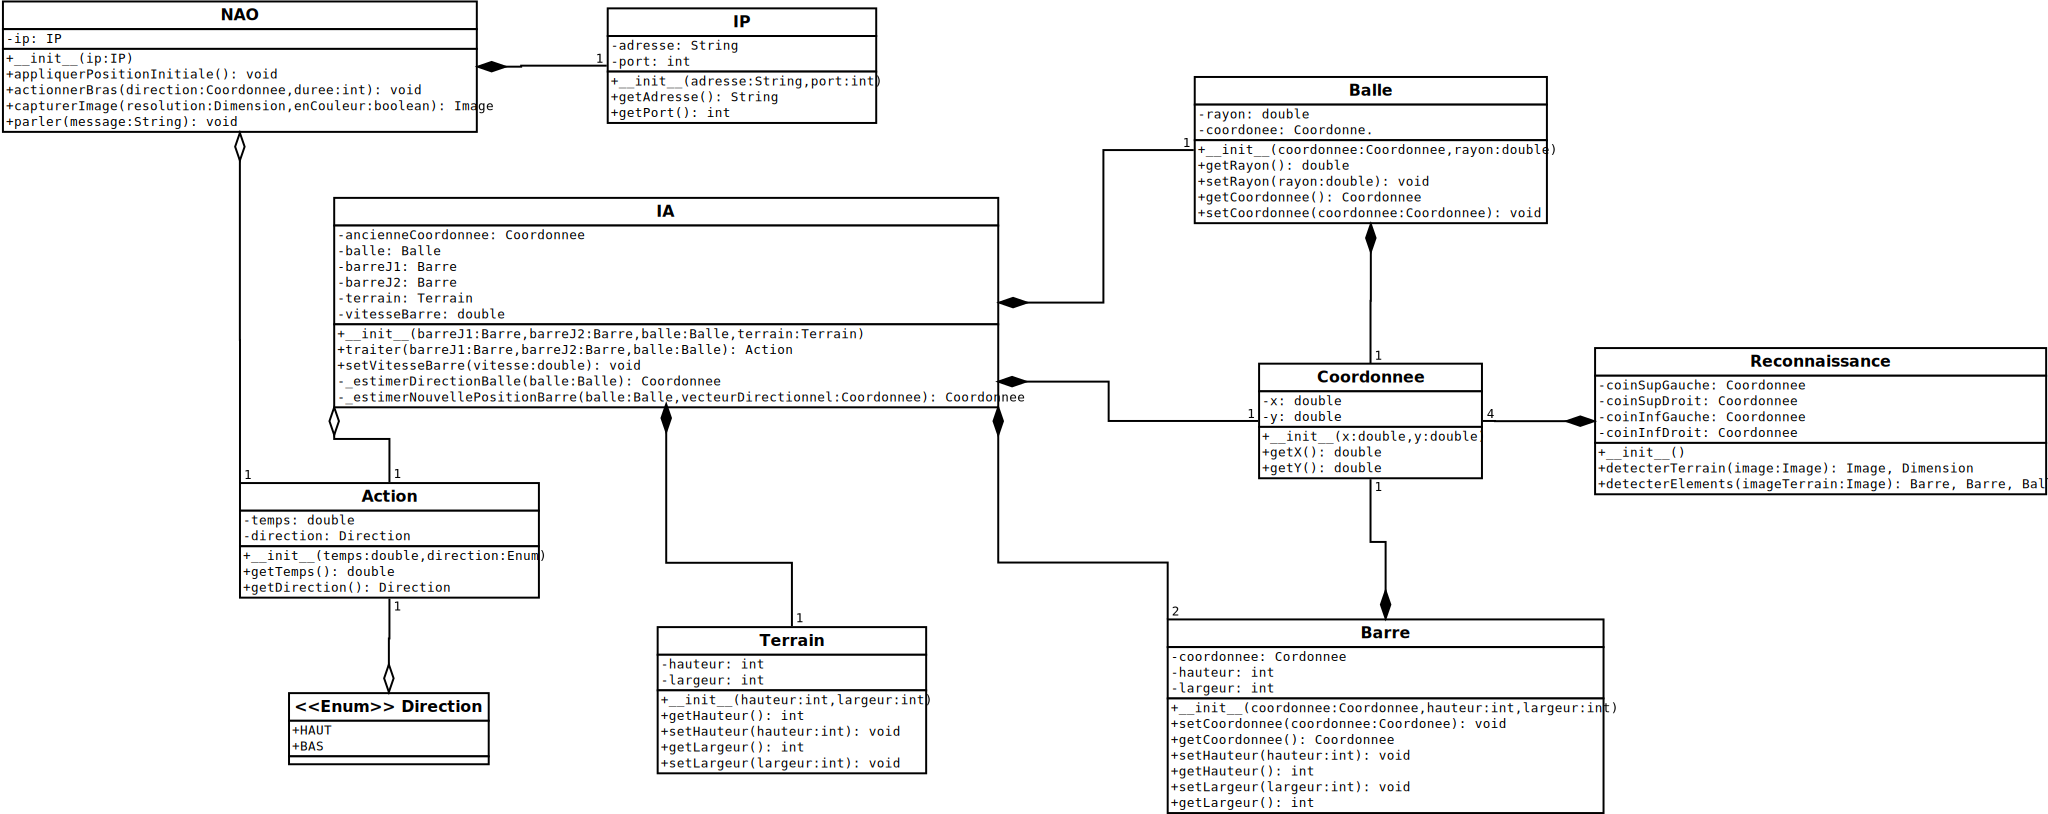
\includegraphics[angle=90, height=18cm, width=\textwidth]{Images/DiagrammeDeClasses.png}
  \end{figure}

\newpage

\section{Diagramme de séquence}
\label{sec:Diagramme de séquence}
  \begin{figure}[!h]
    \caption{Diagramme de séquence}
    \centering
    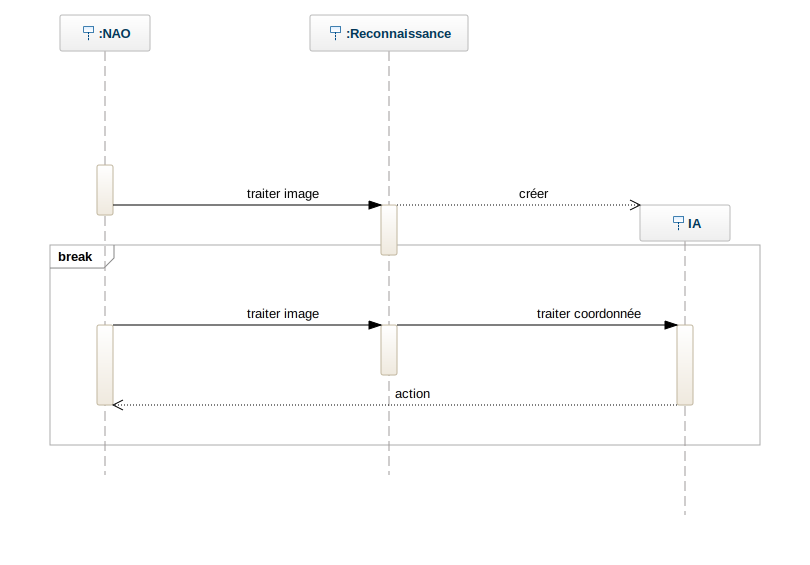
\includegraphics[width=\textwidth]{Images/DiagrammeDeSequence.png}
  \end{figure}



\end{document}
